% !TEX encoding = Windows Cyrillic
\documentclass[a4paper,12pt]{article}
\usepackage[mag=1000]{newlistok}
\usepackage{tikz}
\usetikzlibrary{arrows.meta,positioning}
\usetikzlibrary{calc}

\УвеличитьШирину{1.4truecm}
\УвеличитьВысоту{2.5truecm}

\Заголовок{Потоки на графах}
\НомерЛистка{13д}
%\renewcommand{\spacer}{\vfill}
\ДатаЛистка{07.10.2019}
%\Оценки{}

\newcommand{\0}[1]{\overline{#1}}

%\documentstyle[11pt, russcorr, listok]{article}
%\newcommand{\del}{\mathrel{\raisebox{-.3 ex}{${\vdots}$}}}

\begin{document}

\СоздатьЗаголовок
\noindent
{\small Мы будем изучать \выд{потоки} на графах. 
Мы хотим смоделировать поток жидкости по системе труб, или электрического тока по проводам, или автомобилей по дорогам из одной точки в другую.
}




\опр
\выд{Транспортной сетью} или просто \выд{сетью} называется ориентированный граф\footnote{ Формальное определение такое: $V$ --- конечное множество вершин, $E$ --- множество упорядоченных пар вершин, запись $(x,y) \in E$ означает, что есть ребро с началом в $x$ и концом в $y$. В графе могут быть ребра $(x,y)$ и $(y,x)$, но не допускаются кратные рёбра и петли.}\\ $G = (V,E)$, в котором выделены две вершины: \выд{источник} $s$ и \выд{сток} $t$, и для каждого ребра $(x,y) \in E$ заданы \выд{пропускные способности} --- неотрицательные числа $c(x,y)$. Пропускная способность ребра $(x,y)$ задаёт максимальное количество <<жидкости>> или <<тока>>, которая может перетечь из $x$ в $y$.
\копр

{\bf Задача о минимальном разрезе}

Предположим, что нам надо <<отрезать>> источник от стока, затратив при этом минимальные усилия. Считается, что на разрез одного ребра уходит столько сил, какова пропускная способность этого ребра. Формально, {\it разрезом транспортной сети} $[A,\ B]$ назовём такое разбиение\footnote{ $A \sqcup B$ означает, что $A \cup B = V$ и $A \cap B = \emptyset$.} вершин графа $V = A \sqcup B$, что $s\in A$, $t\in B$. \выд{Пропускная способность разреза} $с([A,\ B]) = \sum_{x \in A, y \in B} c(x,y)$ --- сумма пропускных способностей рёбер, идущих из $A$ в $B$.


\УстановитьГраницы{0cm}{8cm}

\задача Для транспортной сети $G_1$ найдите разрез пропускной способности \пункт $62$; \пункт $30$; \пункт меньше $30$. 
\кзадача



\задача Пусть $[A,\ B]$ и $[C,\ D]$ --- два разреза минимальной пропускной способности. Являются ли минимальными разрезы $[A \cup C, \overline{A \cup C}]$ и  $[A \cap C, \overline{A \cap C}]$?
\кзадача

\задача[Теорема о бутылочном горлышке]\label{T:BN} \пункт Для каждого разреза $[A,\ B]$ транспортной сети найдём ребро из $A$ в $B$ максимальной пропускной способности, и из получившихся чисел выберем наименьшее: 
\vspace*{-1mm}
$$ \hspace{-5cm}\underline{c} = \min_{[A,\ B]} \max_{x \in A, y \in B}  c(x,y).$$ 

Найдите $\underline{c}$ для транспортных 
сетей $G_1$,$G_2$.

\пункт Пусть $W$ --- множество путей из $s$ в $t$. Для каждого пути  $w \in W$ транспортной сети найдём ребро минимальной пропускной способности, и из получившихся чисел выберем наибольшее: $\overline{c} = \max_{w \in W} \min_{e \in w}  c(e)$. Найдите $\overline{c}$ для транспортных сетей $G_1$, $G_2$.
\пункт Докажите в общем случае, что $\underline{c}=\overline{c}$.
\кзадача
\ВосстановитьГраницы

\vspace{-9.5cm}
\hspace{10.5cm}
  \begin{tikzpicture}[
      mycircle/.style={
         circle,
         draw=black,
         fill=gray,
         fill opacity = 0.3,
         text opacity=1,
         inner sep=0pt,
         minimum size=20pt,
         font=\small},
      myarrow/.style={-Stealth},
      node distance=1.3cm and 1.3cm
      ]
      \node[mycircle] (c1) {$s$};
      \node[mycircle,below right=of c1] (c4) {$v_3$};
      \node[mycircle,right=of c1] (c3) {$v_2$};
      \node[mycircle,above right=of c1] (c2) {$v_1$};
      \node[mycircle,below right=of c3] (c7) {$v_6$};
      \node[mycircle,right=of c3] (c6) {$v_5$};
      \node[mycircle,above right=of c3] (c5) {$v_4$};
      \node[mycircle,right=of c6] (c8) {$t$};


    \foreach \i/\j/\txt/\p in {% start node/end node/text/position
      c1/c2/10/above,
      c1/c4/15/above,
      c1/c3/5/above,
      c2/c3/4/above,
      c3/c4/4/above,
      c2/c5/9/above,
      c2/c6/15/above,
      c3/c6/8/above,
      c7/c3/6/above,
      c4/c7/30/below,
      c5/c6/15/above,
      c6/c7/15/above,
      c5/c8/10/above,
      c6/c8/10/above,
      c7/c8/10/below}
       \draw [myarrow] (\i) -- node[sloped,font=\small,\p] {\txt} (\j);
     \node [below=1cm, align=flush center,text width=8cm] at (3,-1.2)
        {
            Сеть $G_1$
        };
     % draw this outside loop to get proper orientation of 10
    
    \end{tikzpicture}
\hspace*{12cm}
    \begin{tikzpicture}[
      mycircle/.style={
         circle,
         draw=black,
         fill=gray,
         fill opacity = 0.3,
         text opacity=1,
         inner sep=0pt,
         minimum size=20pt,
         font=\small},
      myarrow/.style={-Stealth},
      node distance=0.6cm and 1.2cm
      ]
      \node[mycircle] (c1) {$s$};
      \node[mycircle,below right=of c1] (c2) {$v_2$};
      \node[mycircle,right=of c2] (c3) {$v_4$};
      \node[mycircle,above right=of c1] (c4) {$v_1$};
      \node[mycircle,right=of c4] (c5) {$v_3$};
      \node[mycircle,below right=of c5] (c6) {$t$};

    \foreach \i/\j/\txt/\p in {% start node/end node/text/position
      c1/c2/8/below,
      c1/c4/11/above,
      c2/c3/11/below,
      c3/c6/4/below,
      c4/c5/12/above,
      c5/c6/15/above,
      c5/c2/4/below,
      c3/c5/7/below,
      c2.70/c4.290/1/below}
       \draw [myarrow] (\i) -- node[sloped,font=\small,\p] {\txt} (\j);

     % draw this outside loop to get proper orientation of 10
     \draw [myarrow] (c4.250) -- node[sloped,font=\small,above,rotate=180] {10} (c2.110);
        \node [below=1cm, align=flush center,text width=8cm] at (3,-0.5)
        {
            Сеть $G_2$
        };
    \end{tikzpicture}

\vspace{0.5cm}


Как показывает задача \ref{T:BN}, вопросы о разрезах связаны с <<пропускными способностями>> путей из источника в сток. Чтобы оценить пропускные способности набора путей, введём понятие потока.


\опр
\выд{Потоком} на транспортной сети называется способ написать на всех рёбрах \выд{потоки } --- такие числа $f(x,y)$, что выполняются два свойства:
\begin{nums}{-2}
	\item для всех вершин, кроме источника и стока, сумма потоков входящих рёбер равна сумме потоков исходящих рёбер. В виде формулы это условие можно записать так:  $$\mbox{ если $y$ --- не источник, и не сток, то} \sum_{x : (x,y) \in E} f(x,y) = \sum_{z : (y,z) \in E} f(y,z);$$
	\item поток каждого ребра неотрицателен и не превышает его пропускную способность: $$0 \leq f(x,y) \leq c(x,y).$$
\end{nums}

\выд{Величиной потока} $v(f)$ называют сумму потоков из источника.
\копр

\задача Для сети $G_1$ постройте поток величиной числа $\alpha$, где \пункт $\alpha \leq 24$; \пункт $\alpha \leq 28$.
\кзадача




\опр 
\выд{Поток через разрез } --- сумма всех потоков из вершины, лежащей в $A$ в вершину, лежащую в $B$ минус сумма всех потоков из вершин, лежащих в $B$, в вершину, лежащую в $A$, то есть $f(A,B)-f(B,A)= \sum_{x \in A, y \in B} f(x,y) -  \sum_{x \in A, y \in B} f(y,x)$.
\копр


\задача Докажите, что 
\пункт для любого разреза $[A,B]$ поток через разрез равен величине потока: $v(f) = f(A,B)-f(B,A)$.
\пункт величина потока равна сумме потоков в сток, то есть $$v(f) = \sum_{x: (x,t) \in E} f(x,t).$$
\кзадача

\задача \пункт Докажите, что величина произвольного потока не превосходит пропускной способности любого разреза.   \пункт Найдите поток максимальной величины и разрез минимальной пропускной способности сети $G_1$.
\кзадача

В следующей задаче мы приводим идею по построению  \выд{максимального потока} (потока с максимальной величиной).

\УстановитьГраницы{0cm}{8cm}

\задача Предположим, что нам дана транспортная сеть с пропускной способностью $c(x,y)$.
\пункт Максимальный поток в сети положителен тогда и только тогда, когда существует путь из источника в сток, проходящий по рёбрам с положительной пропускной способностью.

Попробуем  для имеющегося потока $f(x,y)$ перестроить сеть, чтобы увеличить мощность.
Рассмотрим два определения остаточной сети.

\выд{Остаточная сеть-1}. Это сеть с тем же множеством вершин и рёбер, а пропускная способность ребра из $x$ в $y$ равна $c(x,y)-f(x,y)$.

\выд{Остаточная сеть-2}. Это сеть с тем же множеством вершин, а пропускная способность ребра из $x$ в $y$ равна $c(x,y)-f(x,y)$, а ребра из $y$ в $x$ равна $f(x,y)$. Если ребра из $y$ в $x$ не было, его надо добавить. Если возникло два ребра из $y$ в $x$, то заменим их на одно ребро суммарной пропускной способности.
\ВосстановитьГраницы
\пункт Нарисуйте остаточные сети-1 и -2 для потока, изображённого справа.



\пункт Верно ли, что поток $f$ не является максимальным тогда и только тогда, когда максимальный поток в остаточной сети-1 положителен? остаточной сети-2 положителен?

\пункт Найдите максимальные потоки для сетей, изображённых справа.
 \кзадача

\vspace{-11cm}
\hspace{11.5cm}
 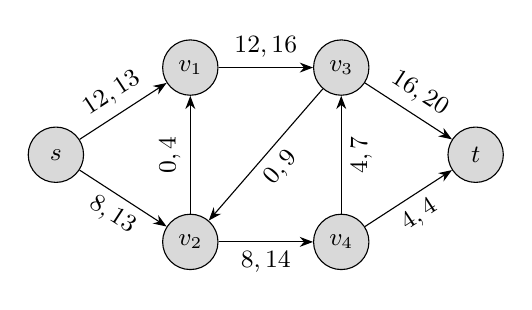
\begin{tikzpicture}[
      mycircle/.style={
         circle,
         draw=black,
         fill=gray,
         fill opacity = 0.3,
         text opacity=1,
         inner sep=0pt,
         minimum size=20pt,
         font=\small},
      myarrow/.style={-Stealth},
      node distance=0.6cm and 1.2cm
      ]
      \node[mycircle] (c1) {$s$};
      \node[mycircle,below right=of c1] (c2) {$v_2$};
      \node[mycircle,right=of c2] (c3) {$v_4$};
      \node[mycircle,above right=of c1] (c4) {$v_1$};
      \node[mycircle,right=of c4] (c5) {$v_3$};
      \node[mycircle,below right=of c5] (c6) {$t$};

    \foreach \i/\j/\txt/\p in {% start node/end node/text/position
      c1/c2/{$8,13$}/below,
      c1/c4/{$12,13$}/above,
      c2/c4/{$0,4$}/above,
      c5/c2/{$0,9$}/below,
      c2/c3/{$8,14$}/below,
      c3/c6/{$4,4$}/below,
      c4/c5/{$12,16$}/above,
      c5/c6/{$16,20$}/above,
      c3/c5/{$4,7$}/below}
       \draw [myarrow] (\i) -- node[sloped,font=\small,\p] {\txt} (\j);

    \end{tikzpicture}
    
    \vspace{0.5cm}
    \hspace*{11.5cm}
    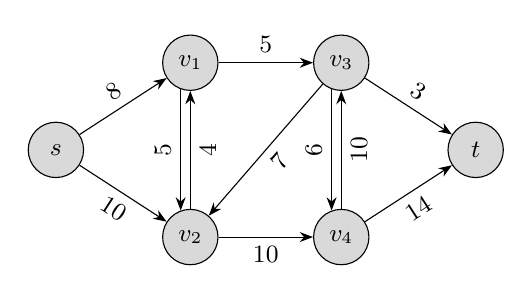
\begin{tikzpicture}[
      mycircle/.style={
         circle,
         draw=black,
         fill=gray,
         fill opacity = 0.3,
         text opacity=1,
         inner sep=0pt,
         minimum size=20pt,
         font=\small},
      myarrow/.style={-Stealth},
      node distance=0.6cm and 1.2cm
      ]
      \node[mycircle] (c1) {$s$};
      \node[mycircle,below right=of c1] (c2) {$v_2$};
      \node[mycircle,right=of c2] (c3) {$v_4$};
      \node[mycircle,above right=of c1] (c4) {$v_1$};
      \node[mycircle,right=of c4] (c5) {$v_3$};
      \node[mycircle,below right=of c5] (c6) {$t$};

    \foreach \i/\j/\txt/\p in {% start node/end node/text/position
      c1/c2/{$10$}/below,
      c1/c4/{$8$}/above,
      c2.90/c4.270/{$4$}/below,
      c5/c2/{$7$}/below,
      c2/c3/{$10$}/below,
      c3/c6/{$14$}/below,
      c4/c5/{$5$}/above,
      c5/c6/{$3$}/above,
      c3.90/c5.270/{$10$}/below}
       \draw [myarrow] (\i) -- node[sloped,font=\small,\p] {\txt} (\j);

\draw [myarrow] (c4.250) -- node[sloped,font=\small,above,rotate=180] {5} (c2.110);
\draw [myarrow] (c5.250) -- node[sloped,font=\small,above,rotate=180] {6} (c3.110);


    \end{tikzpicture}

\vspace{3.5cm}

\задача Для потока $F$ на транспортной сети следующие условия эквивалентны:

(1) $F$ --- максимальный поток;

(2) В остаточной сети потока $F$ нет потока положительной величины.

(3) Существует разрез пропускной способности $v(f)$.

\кзадача

\задача[теорема Форда-Фалкерсона] Наименьшая пропускная способность разреза равна величине максимального потока.
\кзадача


\задача Предположим, что пропускные способности всех рёбер в сети --- целые числа.

\пункт Опишите алгоритм, позволяющий находить максимальный поток в этой сети. Проверьте, что алгоритм в какой-то момент остановится, а не будет работать бесконечно долго. Этот алгоритм называется алгоритмом Форда-Фалкерсона.

\пункт Докажите, что в сети существует целочисленный поток, то есть поток, в котором величина потока на любом ребре целая.
\УстановитьГраницы{0cm}{8cm}
\пункт Существует ли сеть такого вида с нецелочисленным 
максимальным потоком?

\пункт Можно ли обобщить результат пункта а) на случай рациональных пропускных способностей?

\кзадача



\задача Докажите, что для графа на рисунке справа алгоритм Форда-Фалкерсона будет работать бесконечно долго. Здесь $b = \frac{\sqrt{5}-1}{2}$. \кзадача

\ВосстановитьГраницы

\vspace{-4cm}
\hspace{11.5cm}
    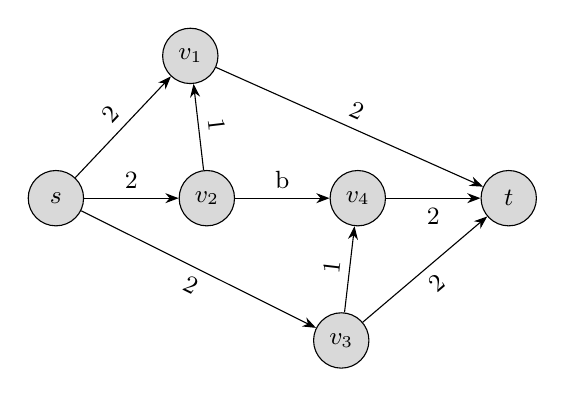
\begin{tikzpicture}[
      mycircle/.style={
         circle,
         draw=black,
         fill=gray,
         fill opacity = 0.3,
         text opacity=1,
         inner sep=0pt,
         minimum size=20pt,
         font=\small},
      myarrow/.style={-Stealth},
      node distance=1.3cm and 1.2cm
      ]
      \node[mycircle] (c1) {$s$};
      \node[mycircle,above right=of c1] (c2) {$v_1$};
      \node[mycircle,right=of c1] (c3) {$v_2$};
      \node[mycircle,below right=of c3] (c4) {$v_3$};
      \node[mycircle,right=of c3] (c5) {$v_4$};
      \node[mycircle,right=of c5] (c6) {$t$};

    \foreach \i/\j/\txt/\p in {% start node/end node/text/position
      c3/c2/1/above,
      c4/c5/1/above,
      c3/c5/b/above,
      c1/c2/2/above,
      c1/c3/2/above,
      c1/c4/2/below,
      c2/c6/2/above,
      c5/c6/2/below,
       c4/c6/2/below}
       \draw [myarrow] (\i) -- node[sloped,font=\small,\p] {\txt} (\j);

     \end{tikzpicture}

%\GenXMLW
\ЛичныйКондуит{0mm}{6mm}

\end{document}


\задача Предположим, что мы уберём условие целочисленности из определения потока. Верно ли, что в этом случае максимальный поток будет целочисленным на каждом ребре?
\кзадача

\задача[теорема Менгера о рёберной связности] Выберем в неориентированном графе две различные вершины $x$ и $y$. Тогда следующие две величины равны:
\begin{itemize}
	\item максимальное количество непересекающихся по рёбрам путей между $x$ и $y$;
	\item минимальное количество рёбер, после удаления которого от $x$ нельзя будет дойти до $y$.
\end{itemize}
\кзадача

\опр
Подмножество $S$ множества вершин графа называется \выд{вершинным сепаратором} для несмежных вершин $x$ и $y$, если удаление $S$ разделяет $x$ и $y$ в разные компоненты связности.
\копр

\задача[теорема Менгера о вершинной связности] Выберем в неориентированном графе две различные не соединённые ребром вершины $x$ и $y$. Тогда следующие две величины равны:
\begin{itemize}
	\item максимальное количество непересекающихся по вершинам вне $x$ и $y$ путей между $x$ и $y$;
	\item размер минимального вершинного сепаратора для $x$ и $y$.
\end{itemize}
\footnotesize{Указание: замените каждую вершину, кроме $x$ и $y$, на две, соединённые ребром.}
\кзадача

\задача
Рассмотрим двудольный граф $G$ с долями $X$ и $Y$. Назовём \выд{вершинным покрытием} набор вершин такой, что любое ребро имеет хотя бы одну конечную вершину из этого набора.
\пункт Добавим к графу $G$ вершины $s$ и $t$, соединённые со всеми вершинами из $X$ и $Y$ соответственно. Докажите, что размер минимального вершинного покрытия равен размеру минимального вершинного сепаратора для $s$ и $t$.
\пункт Превратим граф из предыдущего пункта в сеть, сделав $s$ источником, а $t$ --- стоком, и нарисовав стрелочки из $X$ в $Y$. Придумайте пропускные способности таким образом, чтобы выполнялся такой факт: если в $F$ есть сечение пропускной способности $k$, то в $G$ есть вершинное покрытие из $k$ вершин.
\пункт[теорема Кёнига] В двудольном графе размер минимального вершинного покрытия равен размеру максимального \выд{паросочетания}, то есть набора рёбер без общих вершин.
\кзадача

\задача[теорема Холла]
В некоторой компании $n$ юношей. При каждом $k$ от 1 до $n$ верно утверждение: для любых $k$ юношей в компании число девушек, знакомых хотя бы с одним из этих $k$ юношей, не меньше k. Можно ли женить всех юношей на знакомых девушках?
\кзадача
\задача
\пункт Рассмотрим сеть (как обычно, ориентированный граф со стоком и источником), в которой на каждом ребре $(x,\ y)$ написаны два числа: верхняя и нижняя пропускная способность $u(x,\ y)$ и $l(x,\ y)$. Потоком в такой сети будем называть такой способ сопоставить каждому ребру поток по нему, что он не меньше нижней пропускной способности и не больше верхней. Пусть в этой сети есть хотя бы один поток. Докажите, что тогда найдётся такой поток $f$ и сечение $A,\ B$, что выполняются два условия:
\begin{enumerate}
	\item для любого ребра $(x,y)$ такого, что $x\in A, y\in B$, выполнено $f(x,y)=u(x,y)$
	\item для любого ребра $(x,y)$ такого, что $x\in B, y\in A$, выполнено $f(x,y)=l(x,y)$
\end{enumerate}
Выведите отсюда предыдущую формулировку теоремы Форда-Фалкерсона.

\пункт Рассмотрим сеть в смысле предыдущего пункта со всеми нижними пропускными способностями, равными $-\infty$ и хотя бы одним конечным сечением. Докажите, что для минимального сечения $A,\ B$ нет путей из $B$ в $A$.
\пункт[теорема Дилуорса] Рассмотрим ориентированный граф без циклов. Докажите, что следующие величины равны:
\begin{itemize}
	\item размер минимального набора путей, содержащего все вершины
	\item размер максимального множества, не содержащего пары вершин такой, что от одной вершины можно дойти до другой.
\end{itemize}
\кзадача

% \GenXMLW

\ЛичныйКондуит{0mm}{6mm}

\end{document}
